\subsubsection{Wersja YAML}
Cała struktura zadań podzielona jest na kilka grup - tworząc je możemy zacząć od etapów (ang. stage), 
wewnątrz nich zawrzeć kilka jobów (prac, zadań), które składają się z kroków wykonania (ang. steps).

\begin{figure}[ht]
    \centering
    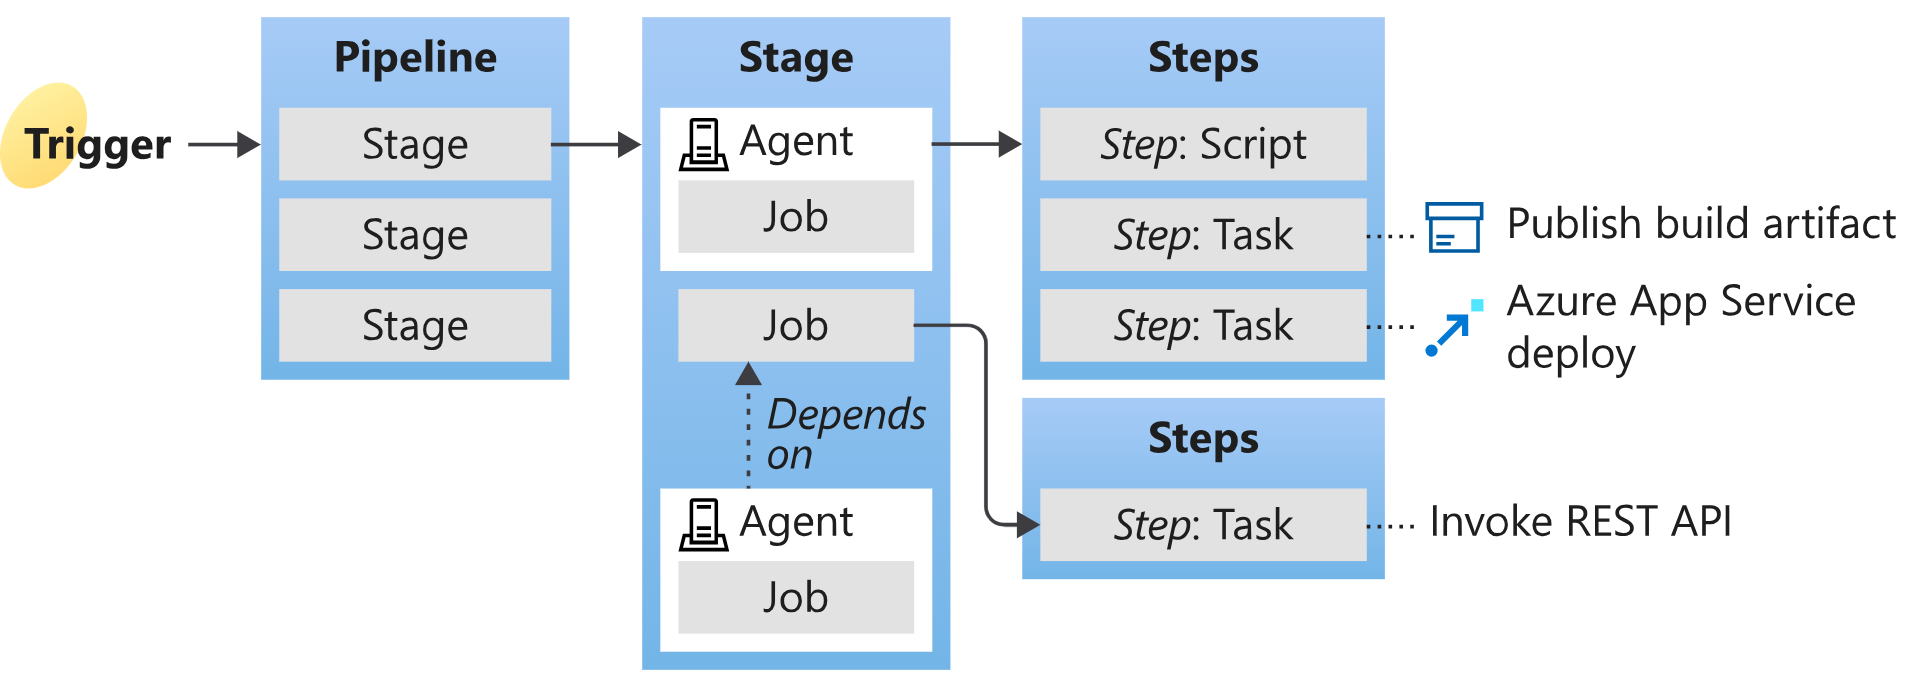
\includegraphics[width=\textwidth]{pipelineSchemaAzure.png}
    \caption{Hierarchia etapów i zadań w Azure~\cite{pipelineSchemaAzure_source}}
    \label{img:pipelineSchemaAzure}
\end{figure}
Finalną wersję pipeline'a umieściłem bezpośrednio w repozytorium jako pliki YAML w folderze \verb|CI|.
Korzystając z możliwości Azure podzieliłem duży plik zawierający wszystkie kroki 
na pomniejsze template'y (szablony), które mogę ponownie wykorzystać w dowolnie dużej 
ilości i kolejności.
Na rysunku~\ref{img:shortFinalCIDiagram} zawarłem skrótowy diagram, który 
przedstawia kolejność wykonywanych etapów działania pipeline'a. 
Zdecydowałem się na wykorzystanie zmiennych do zdefiniowania wersji środowisk potrzebnych 
do kompilacji, ale bez problemu można było parametryzować więcej opcji, jak choćby 
profil kompilacji (przykładowo najpopularniejsze \verb|Debug| lub \verb|Release|) czy 
możliwość publikacji rozwiązania w trybie wersji roboczej (opcja \verb|IsDraft|).

\begin{figure}[hb]
    \centering
    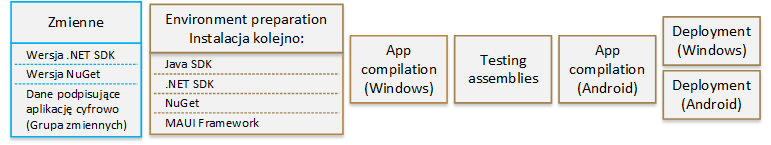
\includegraphics[width=\textwidth]{shortFinalCIDiagram.png}
    \caption{Ogólna logika finalnego pipeline'a}
    \label{img:shortFinalCIDiagram}
\end{figure}

Na rysunku~\ref{img:yamlCompilationDeploymentDiagram} uszczegółowiłem kroki kompilacyjne 
oraz wydawcze z rysunku~\ref{img:shortFinalCIDiagram}. Pozwoliłem sobie nie dodawać kolejnego 
rysunku na etap testowania, ponieważ ogranicza się on do wykonania polecenia \verb|dotnet test|
ze wskazaniem w parametrach ścieżki do projektu testującego 
oraz eksportu wyników tzw. pokrycia kodu testami.

\begin{figure}[ht]
    \centering
    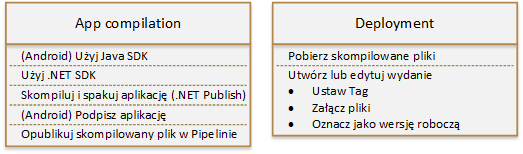
\includegraphics[width=\textwidth]{yamlCompilationDeploymentDiagram.png}
    \caption{Diagram przedstawiający kroki podejmowane wewnątrz kroku AppCompilation oraz Deployment}
    \label{img:yamlCompilationDeploymentDiagram}
\end{figure}

Dla każdego działania pipeline'a możemy zobaczyć podsumowanie wykonanych zadań.
Pierwszym widokiem (rys. \ref{img:runSummary}) jest wypunktowanie podstawowych informacji o podjętej pracy:
\begin{itemize}
    \item Skąd i w jakiej wersji pobraliśmy kodu
    \item Czas trwania oraz data rozpoczęcia działania zadania
    \item Wygenerowane artefakty (skompilowane pliki)
    \item Podsumowanie testowania kodu
\end{itemize}

W bardziej szczegółowych widokach mamy dostęp do analityki (rys. \ref{img:pipelineAnalytics}), 
gdzie możemy sprawdzić wydajność określonych zadań w pipelinie~\footnote{%
    Z uwagi na zmianę umiejscownienia plików wewnątrz repozytorium byłem zmuszony stworzyć 
    nowego pipeline'a w rozumieniu Azure, stąd tak niewielka ilość danych.
}, czy szczegółowego omówienia wykonanych testów (rys. \ref{img:testCoverage}).

\newpage
\newgeometry{left=1cm,top=1cm,bottom=0.3cm}
\begin{figure}[!ht]
    \centering
    \frame{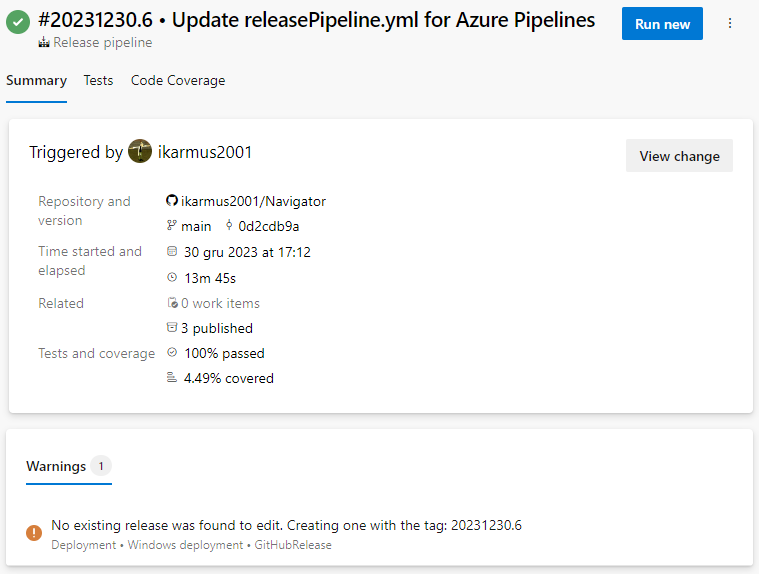
\includegraphics[width=\textwidth]{runSummary_light_2.png}}
    \caption{Ogólne podsumowanie efektu działania pipeline'a}
    \label{img:runSummary}
\end{figure}

\begin{figure}[!ht]
    \centering
    \frame{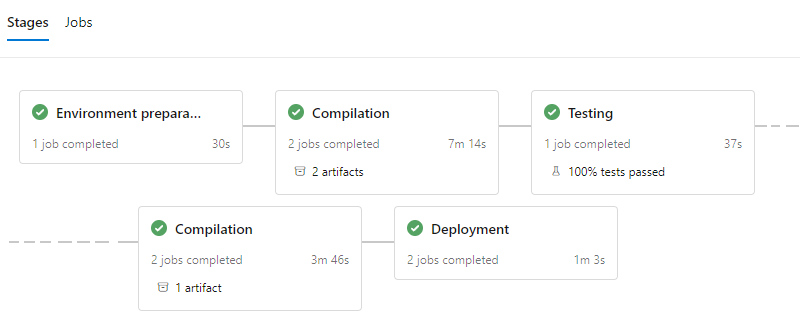
\includegraphics[width=\textwidth]{stagesOverview_light.png}}
    \caption{Spis wykonanych zadań}
    \label{img:stagesOverview}
\end{figure}

\begin{figure}[!ht]
    \centering
    \noindent\frame{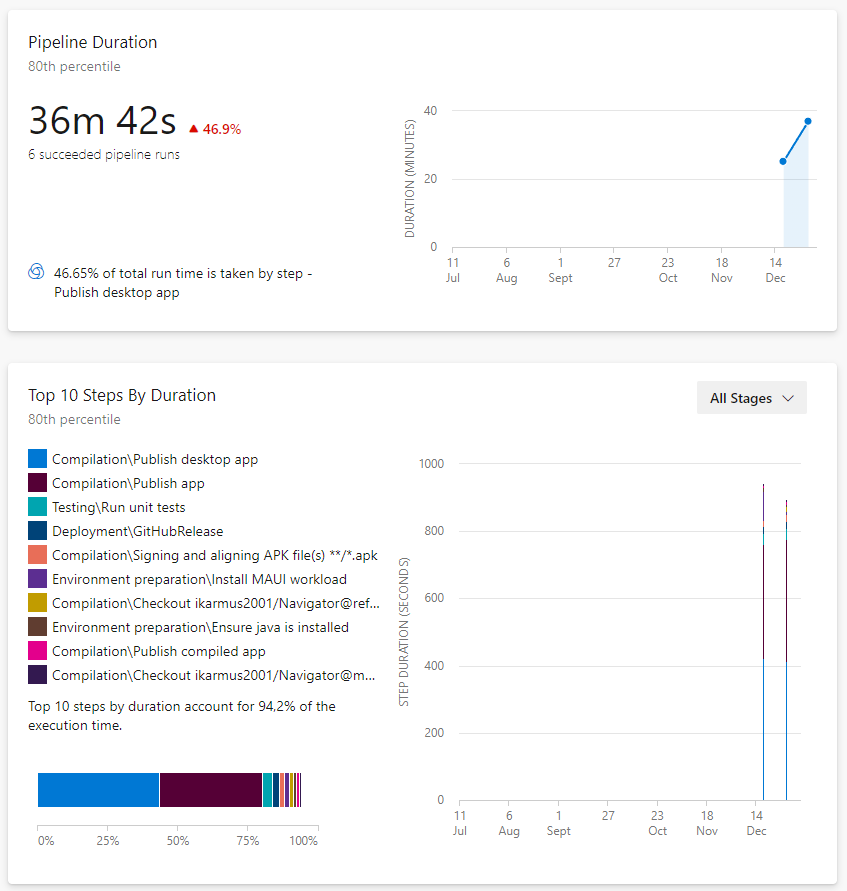
\includegraphics[width=0.95\textwidth]{pipelineAnalytics.png}}
    \caption{Widok analityczny, pozwalający na określenie czasu poświęconego na wykonanie
        określonych zadań w pipelinie}
    \label{img:pipelineAnalytics}
\end{figure}


\begin{figure}[!hb]
    \centering
    \noindent\frame{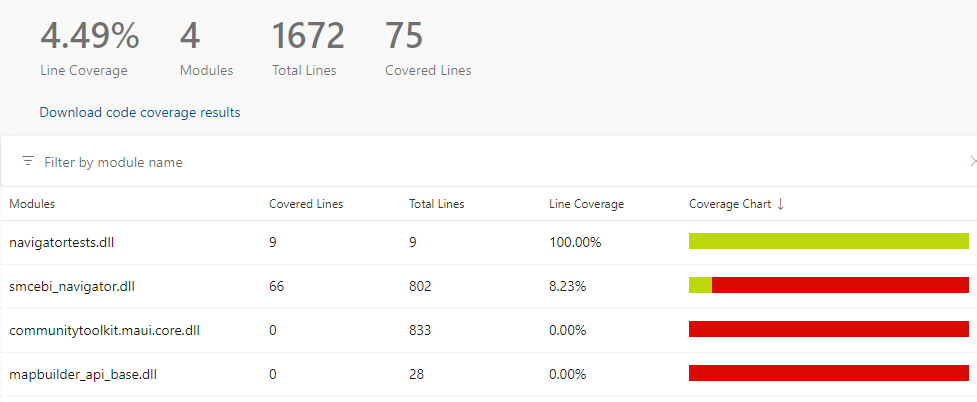
\includegraphics[width=0.95\textwidth]{testCoverage_light.png}}
    \caption{Widok podsumowania testów kodu po kompilacji}
    \label{img:testCoverage}
\end{figure}

\restoregeometry
